\documentclass[aspectratio=1610,xcolor=dvipsnames,t]{beamer} 

\usepackage{listings} 
\usepackage{color} 
\usepackage{xcolor}  
\usepackage{microtype} 
\usepackage{helvet} 
\usepackage{inconsolata} 
\usepackage[framemethod=TikZ]{mdframed} 
\usepackage{graphicx} 
\usepackage{alltt}
\usepackage{sverb} 
\usepackage{verbatim} 

\usetheme{Madrid} 
\useinnertheme{rectangles} 

\setbeamertemplate{navigation symbols}{}
%\setbeamerfont{block title}{size={}}
%\setbeamercolor*{title}{bg=}

%\definecolor{mypurple}{rgb}{.49,0,98}
%\setbeamercolor*{palette primary}{use=structure,fg=white,bg=green}
%\usecolortheme[rgb={0.9,0.2,0.2}]{structure}
\usecolortheme[rgb={0.2,0.7,0.2}]{structure}

\title[Hydrogenic Atoms]{Energy Levels and Spectrum of Hydrogenic Atoms} 
\author{ Michael Papasimeon} 
\date{April 16, 1998}
%\titlegraphic{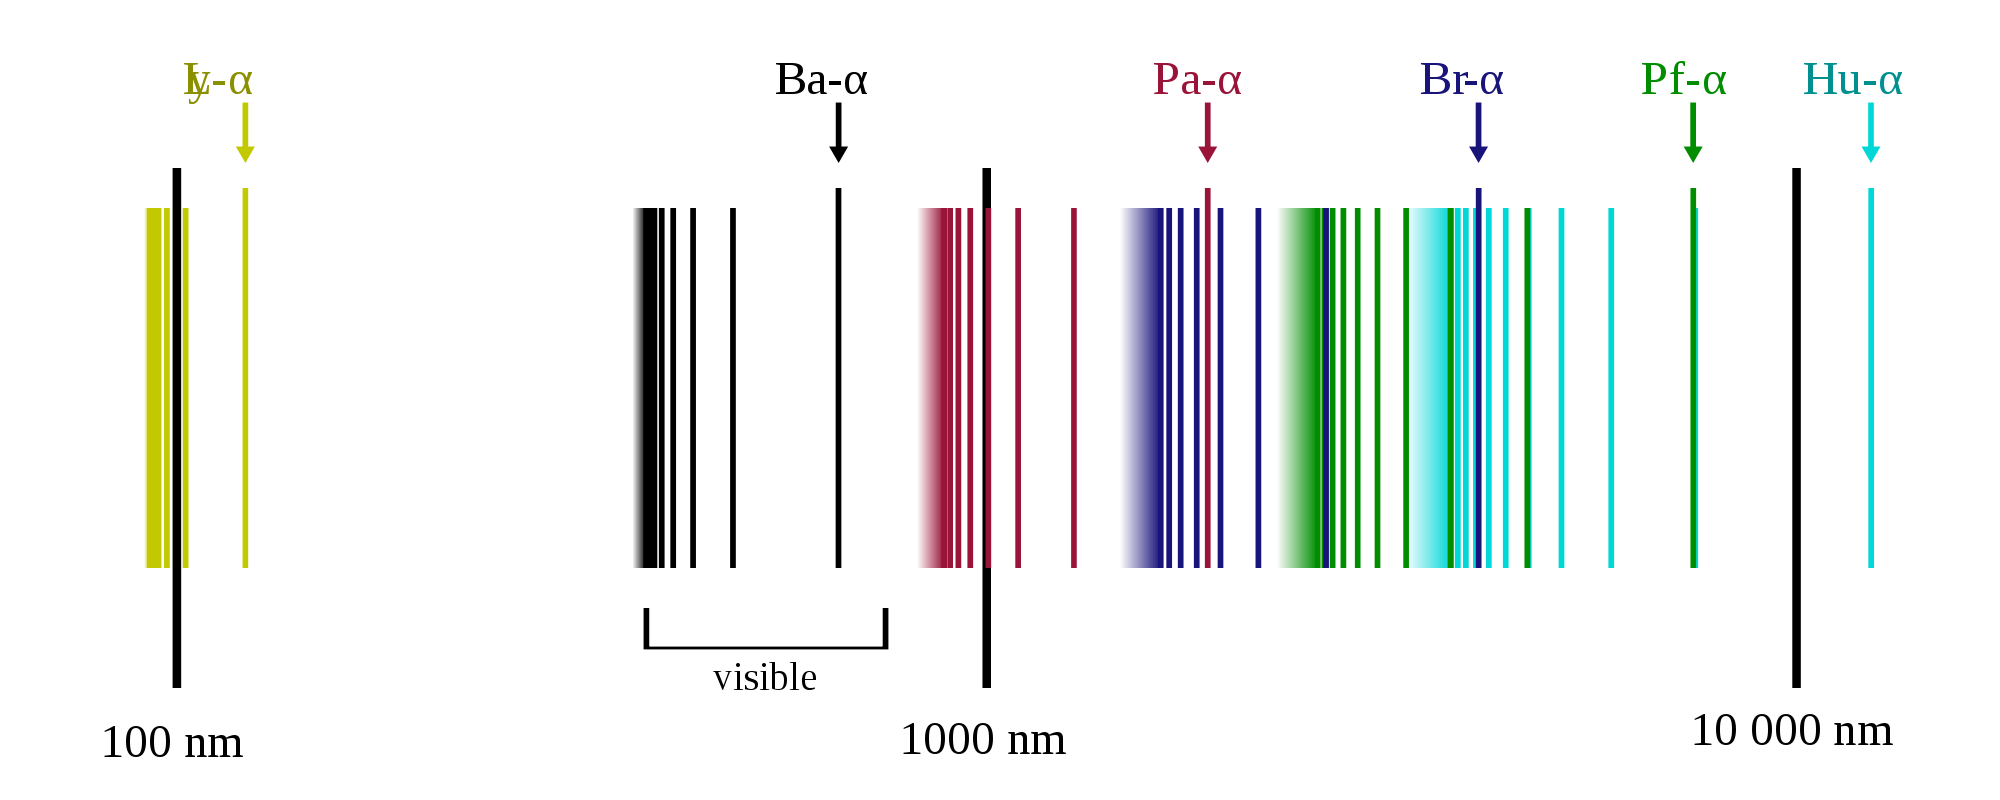
\includegraphics[width=\textwidth]{hydrogen-spectrum}}

\addtobeamertemplate{title
page}{\centering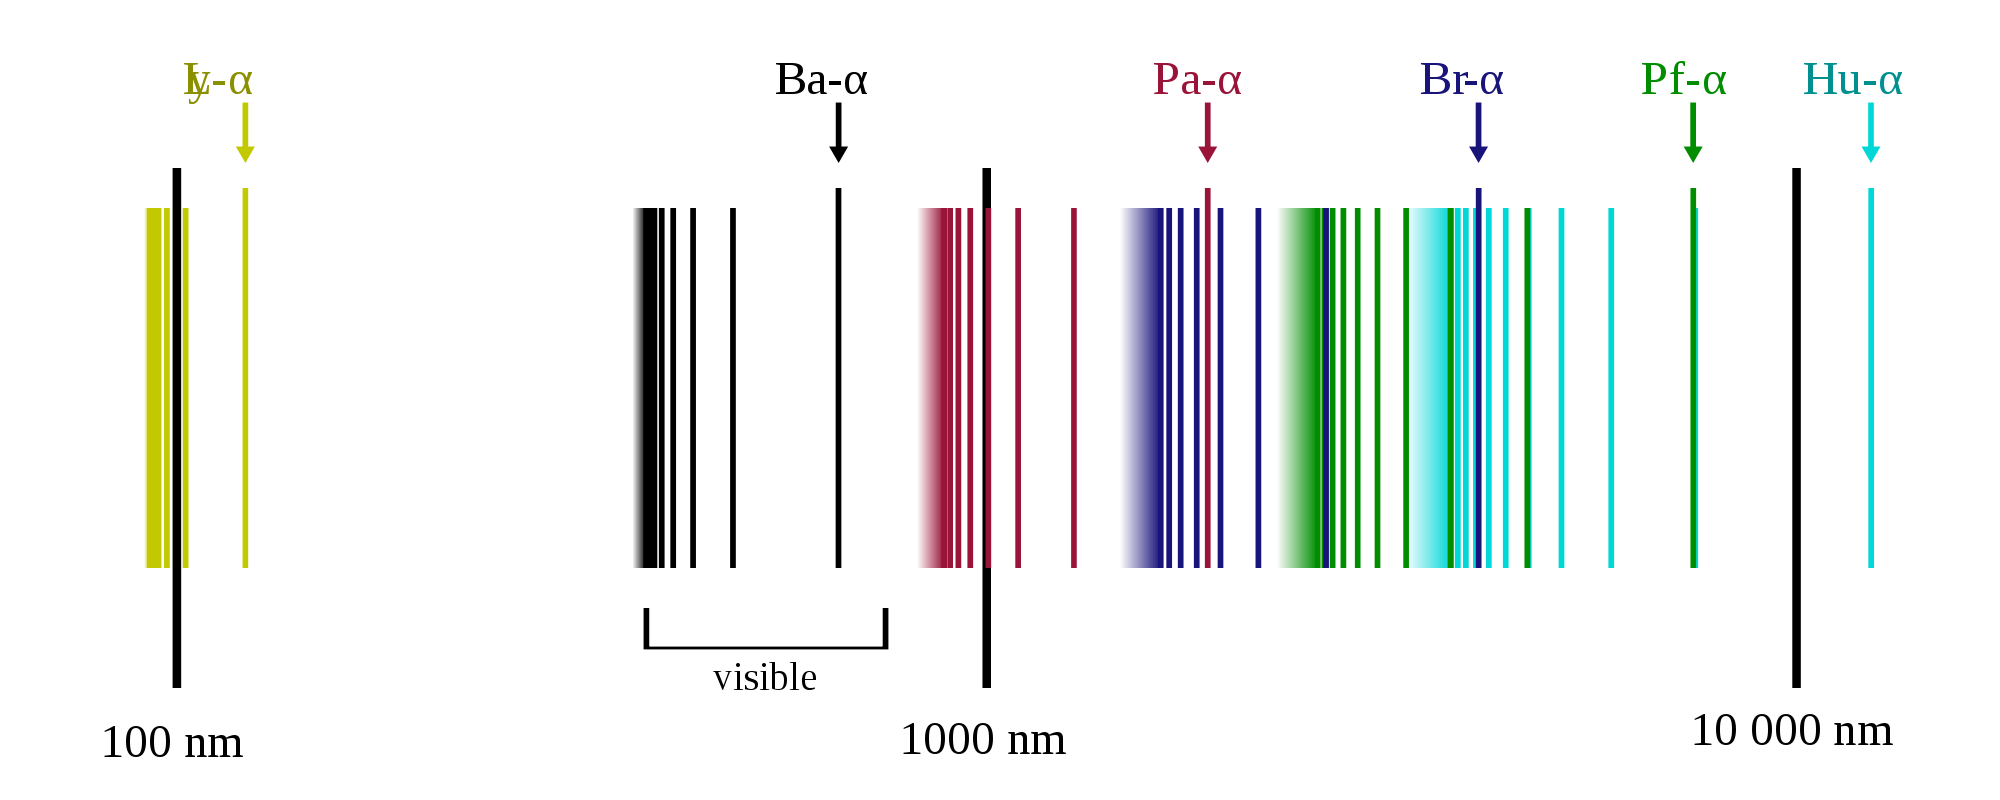
\includegraphics[width=0.5\textwidth]{hydrogen-spectrum}}{}


\newcommand{\ket}[1]{| #1 \rangle}
\newcommand{\bra}[1]{\langle #1 |}
\newcommand{\element}[3]{\bra{#1} #2 \ket{#3}}

\begin{document}

\begin{frame}
    \titlepage
\end{frame} 

\section{Schr\"odinger Equation}

    \subsection{Energy Levels}
    \begin{frame}{Hamiltonian for Electron in Coulomb Potential} 
        A hydrogenic atom can be thought of as an electron with charge ($-e$)
        moving around the spherically symmetric Coulomb potential of the
        nucleus which has charge $Z$. 
        \begin{equation} 
            H = \frac{\bf{p}^2}{2\mu} - \frac{Ze^2}{4 \pi \epsilon_0 r}.
        \end{equation} 
        where $\mu$ is the reduced mass...
        \begin{equation}
            \mu = \frac{Mm}{M + m}
        \end{equation}
    \end{frame} 

    \begin{frame}{Time Independent Schr\"odinger Equation} 
    The problem reduces to solving the time independent Schr\"odinger equation
    for the above Hamiltonian.
    \begin{equation}
    \left[ \frac{{\bf p}^2}{2\mu} - \frac{Ze^2}{4 \pi r}\right] \psi_{nlm} = E_n \psi_{nlm} 
    \end{equation}
    
    \begin{itemize} 
        \item Solving for this equation gives the energy levels of hydrogenic atoms $E_n$, and 
              and corresponding wavefunctions $\psi_{nlm}$. 
        \item The energy levels only depend on the
              principle quantum number $n$, whereas the wavefunctions also depend on the 
              orbital angular momentum quantum number $l$ ($l = 0, 1, ... n - 1$) and 
              magnetic quantum number $m$ ($m = -l, -l + 1, ... , +l - 1, +l$).
    \end{itemize} 
    \end{frame} 

    \begin{frame}{Wave Functions for Hydrogenic Atoms} 
    The wavefunctions of hydrogenic atoms are given by
    \begin{equation}
        \psi_{nlm}({\bf r}) = \psi_{nlm}(r,\theta,\phi)
                           = R_{nl}(r) Y_{lm}(\theta, \phi)
    \end{equation}
    where $R_{nl}(r)$ are the radial wavefunctions and $Y_{lm}(\theta, \phi)$ are
    spherical harmonics. The corresponding energy levels of hydrogenic atoms are
    given by
    \begin{equation}
        E_n = - \frac{1}{2} \mu c^2 \frac{Z^2 \alpha^2}{n^2}
    \end{equation}
    where $\alpha$ is the fine structure constant: 

    $$ \alpha = \frac{e^2}{4 \pi \epsilon_0 \hbar c} $$

    \end{frame} 

    %Since the energy levels depend only on the principle quantum number $n$, we see
    %that the energy levels are degenerate for different values of $l$ and $m$ at a 
    %given value of $n$.
    
    %Figure~\ref{fig:hydrogen-energy} shows the energy levels for the case when $Z = 1$ (Hydrogen).
    %The degeneracy in $l$ can be seen for the different values of $n$.
    %The energy levels shown are known as the gross structure of atomic hydrogen.

    \begin{frame}{Energy Levels of Hydrogen $Z=1$} 
        \centering
        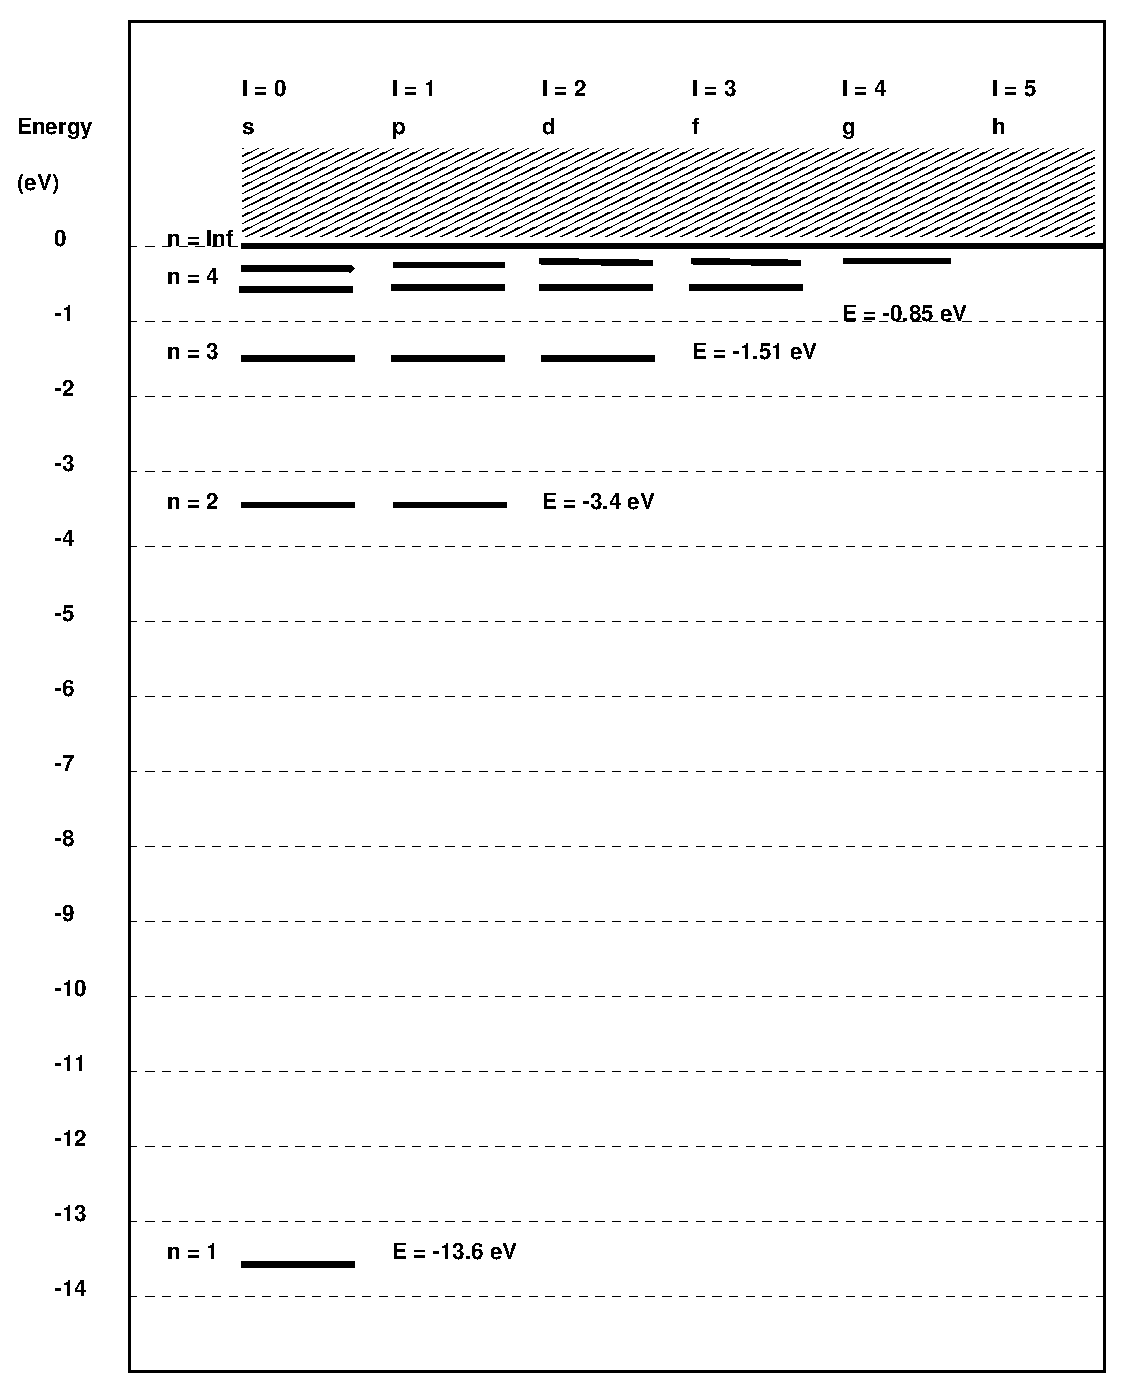
\includegraphics[width=0.4\textwidth]{levels.eps}
    \end{frame} 

    \subsection{Rydberg States}
    \begin{frame}{Rydberg States}  
        \begin{itemize} 
            \item A highly excited hydrogenic atom, that is one with a large principal quantum 
                  number $n$ is said to be known as a \emph{Rydberg Atom}, or to be in a
                  \emph{Rydberg State}.

            \item The Rydberg Atom with $n = 100$, is of an extremely large size -- approximately the size
    of a simple bacteria. However, such an atom has a very small ionisation energy and hence
    the electron is very weakly bound.
        \end{itemize} 
 
    \begin{table} 
        \caption{Bohr orbit radius and binding energy for Hydrogen atoms in 
                 the ground state $n=1$ and Rydberg state $n=100$} 
        \label{tbl:rydberg} 
        \centering
        \begin{tabular}{p{5cm}rr} \hline
            {\bf Quantity}               & $\mathbf{n = 1}$          & $\mathbf{n = 100}$ \\ \hline \hline 
            Bohr Orbit Radius [m]        &  $5.3 \times 10^{-11}$    & $5.3 \times 10^{-7}$ \\ 
            Binding Energy $|E_n|$ [eV]  &  $-13.6 \times 10^0$      & $1.36 \times 10^{-3}$ \\ \hline
        \end{tabular}
    \end{table} 

   \end{frame} 

    \subsection{Hydrogenic Spectrum}
    \begin{frame}{Hydrogenic Spectrum} 
    %Figure~\ref{fig:spectrum} shows the spectrum of atomic hydrogen as predicted by the
    %Bohr model of the atom and by Schr\"odinger's equation. As can be seen there
    %are a number of series of spectral lines -- Lyman, Balmer, Paschen and Brackett.

        \centering
        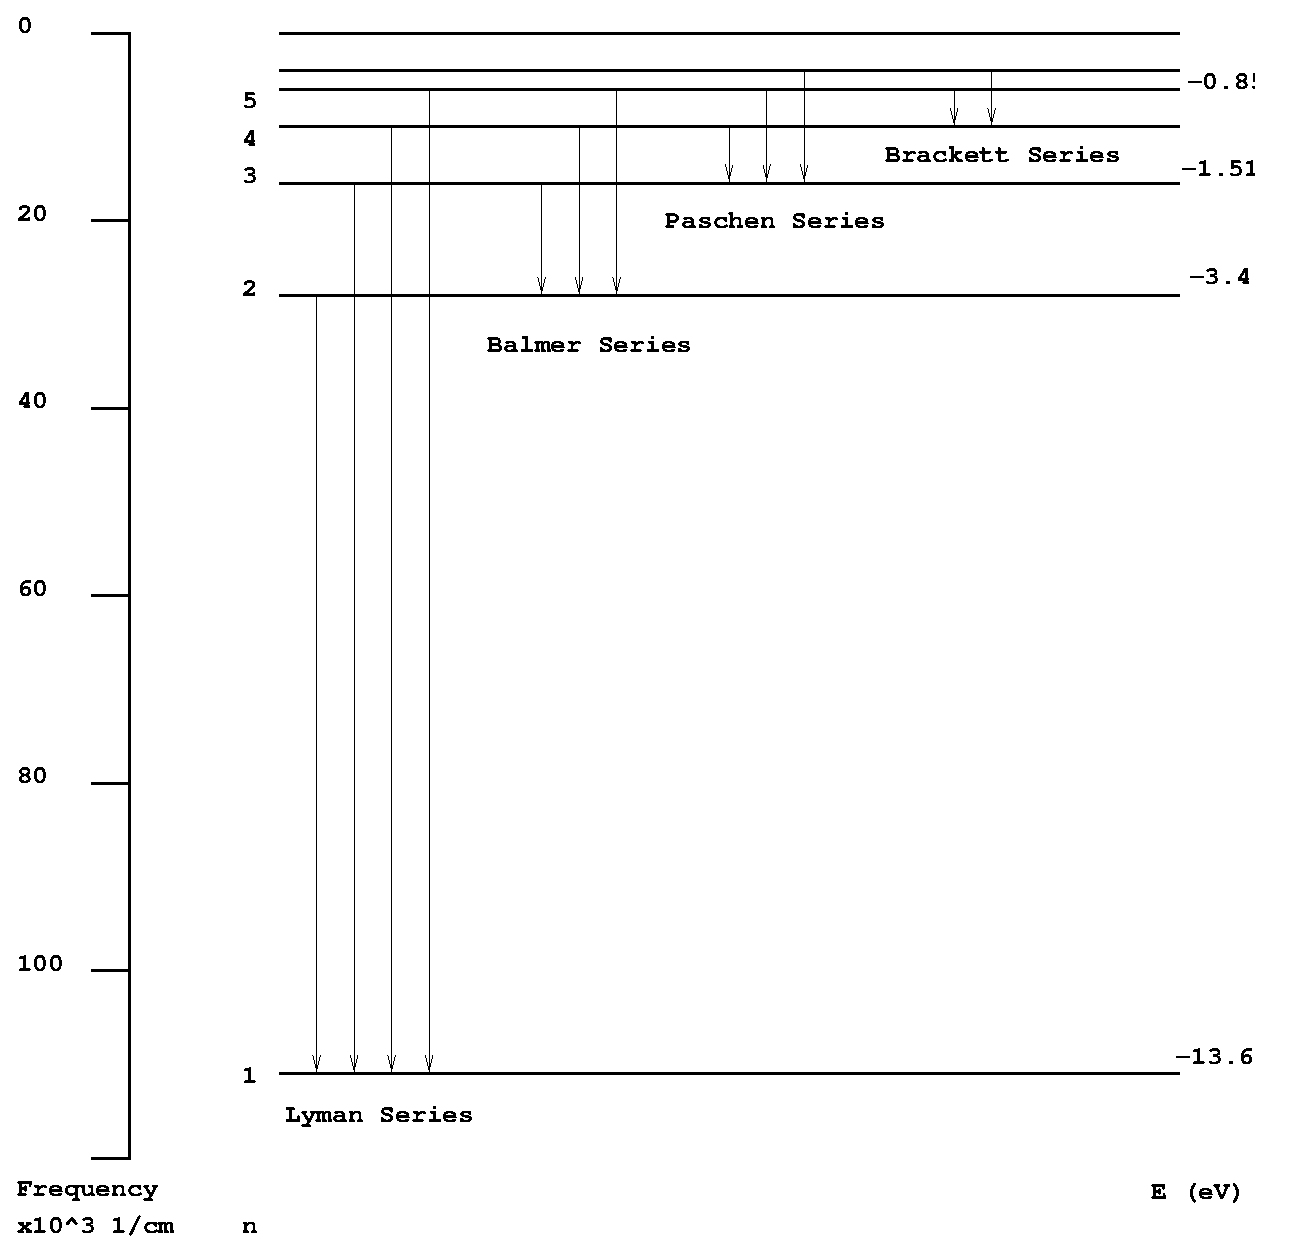
\includegraphics[width=0.6\textwidth]{spectrum}
    \end{frame} 

    \begin{frame}{Lyman, Balmer and Paschen Spectral Lines} 

    %The hydrogen series appear close together in the electromagnetic spectrum.
    %For example, the Lyman Series is in the Ultra-Violet (UV) Region, the Balmer
    %series is in the Visible-UV region and the Paschen, Brackett and Pfund series
    %are in the Infra-Red (IR) Region.

     \begin{table}
        \centering
        %\caption{Lyman, Balmer and Paschen Spectral Lines} 
        \centering
        \begin{tabular}{cc} \hline 
            \multicolumn{2}{c}{\bf Lyman Series (Ultra Violet Region)} \\ \hline 
            Spectral Line & Wavelength (\AA) \\ \hline 
            Ly$_{\alpha}$     &   1216    \\ 
            Ly$_{\beta}$      &   1026    \\ 
            Ly$_{\gamma}$     &   972.5   \\
            Ly$_{\delta}$    &   949.7   \\ \hline 

            \multicolumn{2}{c}{\bf Balmer Series (Visible--Ultra Violet Region)} \\ \hline 
            Spectral Line & Wavelength (\AA) \\ \hline 
            H$_{\alpha}$     &   6563    \\ 
            H$_{\beta}$      &   4861    \\ 
            H$_{\gamma}$     &   4340   \\ \hline 

            \multicolumn{2}{c}{\bf Paschen Series (Infra Red Region)} \\ \hline 
            Spectral Line & Wavelength (\AA) \\ \hline 
            P$_{\alpha}$     &   18751    \\ 
            P$_{\beta}$      &   12818    \\  \hline

        \end{tabular}
    \end{table} 
    \end{frame} 

    %The schematic spectral diagram below shows the Balmer series of atomic
    %hydrogen. It shows the positions of the spectral lines in the electromagnetic
    %spectrum.

    %\begin{figure}[!t] 
    %    \centering
    %    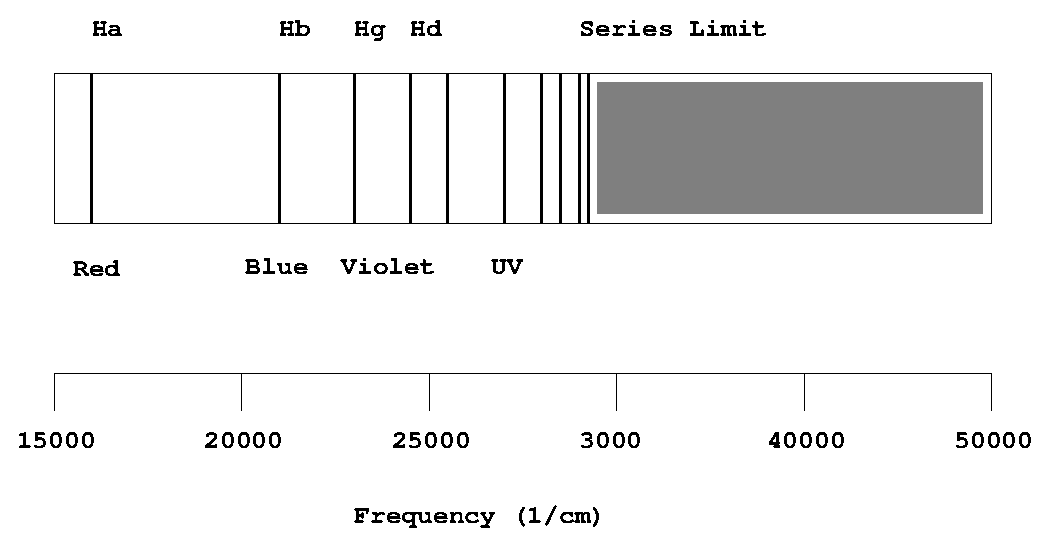
\includegraphics[width=\columnwidth]{balmer}
    %    \caption{Balmer Spectrum for Atomic Hydrogen} 
    %    \label{fig:balmer} 
    %\end{figure} 

\section{Fine Structure}
    \begin{frame}{Fine Structure} 
    %Although the energy levels for hydrogenic atoms shown above agree qualitatively with
    %experiment, very precise measurements of the hydrogen spectrum reveal the existence 
    %a finer structure which can not be explained with the Hamiltonian used above.
    %Experiments reveals that some of the energy levels are split into many smaller levels
    %and therefore many of the degeneracies are lifted.

    \begin{itemize} 

    \item The fine structure of the energy levels of hydrogenic atoms are due to relativistic
    effects and the spin of the electron which were not taken into account in the previous
    section. 
    
    \item We can obtain an estimate on how much the energy levels are shifted, by 
    using perturbation theory if we assume the the relativistic and spin effects are 
    small. We can treat the Hamiltonian, energy eigenfunctions and energy levels as
    the unperturbed case and use first order perturbation theory for the perturbing
    components of the Hamiltonian. 
    \end{itemize} 
    \end{frame} 

    \begin{frame}{Perturbed Hamiltonian for Fine Structure} 
    The Schr\"odinger equation is then of the following form:

    \begin{equation} 
        \left[ H_0 + H'_1 + H'_2 + H'_3 \right] \psi_{nlm} = E \psi_{nlm}
    \end{equation} 

    where $H_0$ corresponds to the unperturbed Hamiltonian used in the previous section,
    and $H'_1$, $H'_2$ and $H'_3$ correspond to small perturbations involving relativistic
    corrections to the kinetic energy, the effect of spin-orbit coupling and the Darwin
    interaction. 
    \end{frame} 
    
    %These three perturbations are described individually below.
    %The process then involves determining the shift in energy to first order for 
    %each of the perturbing terms in the Hamiltonian. 

    \begin{frame}{Modification to Unperturbed Hamiltonian} 
    
    The unperturbed Schr\"odinger 
    equation needs to be slightly modified in order to treat perturbing Hamiltonians
    which take the spin of the electron into account. The modified `unperturbed`
    equation is given by:

    \begin{equation}
        H_0 \psi_{nlm_l m_s }^{(0)} = E_{n}^{(0)} = \psi_{nlm_l m_s}^{(0)} 
    \end{equation}
    where $E_{n}^{(0)}$ are the Schr\"odinger energy eigenvalues (with $\mu = m$) and 
    the zero order wave functions $\psi_{nlm_l m_s}^{(0)}$ are modified two component
    wave functions (also known as Pauli wave functions or spin-orbitals).
    \end{frame} 

    \begin{frame}{Pauli Wave Functions or Spin-Orbitals}  
    \begin{equation}
        \psi_{nlm_l m_s}^{(0)}(q) = \psi_{nlm_l}^{(0)}({\bf r}) \chi_{\frac{1}{2},m_l}
    \end{equation}
    The parameter $q$ represents the combined spin and space coordinate, and 
    $\chi_{\frac{1}{2},m_l}$ are two component spinors (spin eigenfunctions for
    particle of spin one half). 
    \end{frame} 
   
    \begin{frame}{Normalised Spinors} 
    For spin-up ($m_s = +1/2$) and spin-down ($m_s = -1/2$),
    the normalised spinors are denoted by
    \begin{equation}
        \chi_+ = \left( \begin{array}{c}
                    1 \\ 0
                 \end{array} \right)
        \hspace{5mm} \mathrm{and} \hspace{5mm}
        \chi_- = \left( \begin{array}{c}
                    0 \\ 1
                 \end{array} \right)
    \end{equation}

    \begin{itemize} 
        \item Since the unperturbed Hamiltonian does not depend on the spin variable, the
        Pauli wavefunctions are separable in the spin and coordinate variables.
        \item To describe the state of an electron in a hydrogenic atom, we now have the four
        quantum number $n$, $l$, $m_l$ and $m_s$. 
        \item As a result of this, each of the
        unperturbed energy levels are $E_n$ are $2n^2$ degenerate.
    \end{itemize} 
    \end{frame} 

    \begin{frame}{Perturbed Energy Levels} 
    Finally the new perturbed energy levels to first order are given by
    \begin{equation}
        E = E_{n}^{(0)} + \Delta E'_1 + \Delta E'_2 + \Delta E'_3
    \end{equation}
    where $\Delta E'_{(k)}$ is the energy shift resulting from the $k'$th perturbation.
    \end{frame} 
    
	\subsection{Relativistic Correction to the Kinetic Energy}
    \begin{frame}{Relativistic Correction to the Kinetic Energy} 
	\begin{equation}
		H'_1 = - \frac{p^4}{8m^3c^2}
	\end{equation}

    Since relativistic effects were not taken into account previously, the 
    perturbing Hamiltonian $H'_1$ represents the relativistic correction
    to the kinetic energy of the electron.
    Using first order perturbation theory the energy shift is given by
    \begin{equation} 
        \Delta E'_1 = \left \langle nl m_l m_s 
                        \left|
                            \frac{-p^4}{8m^3 c^2} 
                        \right|
                      nl m_l m_s \right \rangle 
    \end{equation}
    \begin{equation}
        \Delta E'_1 = -E_n \frac{Z^2 \alpha^2}{n^2} 
                        \left[ \frac{3}{4}  - \frac{n}{l + \frac{1}{2}} \right]
    \end{equation}
    \end{frame} 

	\subsection{Spin Orbit Interaction}
    \begin{frame}{Spin Orbit Interaction} 
	\begin{equation}
		H'_2 = \frac{1}{2m^2c^2} \frac{1}{r} \frac{dV}{dr} {\bf L} \cdot {\bf S} 
	\end{equation}
    This perturbation corresponds to the shift in the energy as a result of the interaction
    between the internal spin of the electron and it's orbital angular momentum as it
    orbits the nucleus. Since the potential $V(r) = -Ze^2/(4 \pi \epsilon_0 r)$ for
    a hydrogenic atom, the perturbing Hamiltonian becomes
    \begin{equation}
        H'_2 = \frac{1}{2m^2c^2} \frac{Ze^2}{4\pi \epsilon_0 r^3} {\bf L} \cdot {\bf S}
    \end{equation}
    \end{frame} 

    \begin{frame}{Energy Shift for Perturbed Hamiltonian} 
    The energy shift for this perturbing Hamiltonian using first order perturbation theory is
    \begin{equation}
        \Delta E'_2 = -E_n \frac{Z^2 \alpha^2}{2nl(l + \frac{1}{2})(l + 1)}
        \left\{
            \begin{array}{ll}
                l       \mbox{,} &  j = l + \frac{1}{2} \\
                -l - 1  \mbox{,} &  j = l - \frac{1}{2}
            \end{array}
        \right.
    \end{equation}
    \end{frame} 

	\subsection{Darwin Interaction}
    \begin{frame}{Darwin Interaction} 
	\begin{equation}
		H'_3 = \frac{\pi\hbar^2}{2m^2c^2} \left( \frac{Ze^2}{4\pi\epsilon_0} \right) \delta(\bf{r})
	\end{equation}
    The Darwin term does not act on the spin variable and only applies when
    the orbital angular moment is zero ($l=0$).
    The shift energy from the Darwin term is given by
    \begin{equation}
        \begin{array}{ll}
        \Delta E'_3 = -E_n \frac{Z^2 \alpha^2}{n} , & l = 0
        \end{array}
    \end{equation}
    \end{frame} 

    \subsection{Fine Structure Energy Levels to First Order}
    \begin{frame}{Fine Structure Energy Levels to First Order} 
    Based on the energy levels obtained for hydrogenic atoms from the Schr\"odinger equation,
    and the energy shifts obtained from the three perturbation when relativistic and
    spin effects are taken into account we get
    \begin{equation}
        E_{nj} = E_n + \Delta E'_1 + \Delta E'_2 + \Delta E'_3.
    \end{equation}
    Now subtracting from the binding energy $E = mc^2 - E_{nj}$ 
    \begin{equation}
        E = mc^2 \left[ 1 - \frac{(Z \alpha)^2}{2n^2} - \frac{(Z \alpha)^4}{2n^3} 
                        \left(
                            \frac{n}{j + \frac{1}{2}} - \frac{3}{4}
                        \right)
                    \right] 
    \end{equation}
    This result is valid if the perturbation is small, and therefore it begins to break down
    for hydrogenic atoms with large atomic numbers $Z$.
    \end{frame} 

    \subsection{Dirac Equation}
    \begin{frame}{Dirac Equation} 
    The equation which provides the correct energy eigenvalues and eigenstates for
    the fine structure of hydrogenic atoms is the Dirac equation. 
    For a Hydrogenic atom that Dirac equation can be written as:
    \begin{equation}
        \left[ c \mathbf{\alpha} \cdot \mathbf{p} + 
               \beta m c^2 - \frac{Ze^2}{4 \pi \epsilon_0 r}
        \right] \psi = E \psi
    \end{equation}
    where $\psi$ is a 4-component spinor.
    \end{frame} 

    \begin{frame}{Dirac Energy Levels} 
    The Dirac equation takes special relativistic effects and the spin of the electron
    (or any spin-$\frac{1}{2}$ particle) into account, and gives the following solutions for the energy
    eigenvalues for hydrogenic atoms.
    \begin{equation}
        E_{nj}^{Dirac} = \frac{mc^2}
        {
            \sqrt
            { 
                1 + \frac{(Z \alpha)^2}
                {
                    n - j - \frac{1}{2} +
                    \sqrt
                    {
                        \left(j + \frac{1}{2}\right)^2 - (Z \alpha)^2
                    }
                }
            }
        }
    \end{equation}
    Expanding the above equation in a series we obtain
    \begin{equation}
        E = mc^2 \left[ 
            1 - \frac{(Z\alpha)^2}{2n^2} - \frac{(Z\alpha)^4}{2n^2}
                    \left(
                        \frac{1}{j + \frac{1}{2}} - \frac{3}{4n}
                    \right)
                        - ...
                 \right]
    \end{equation}
    This can be seen to agree with the result obtained previously using the perturbation
    theory for the first few terms.
    \end{frame} 

\section{Hyperfine Structure}
    \begin{frame}{Hyperfine Structure} 
        \begin{itemize} 
            \item Until now, the nucleus of hydrogenic atoms has been treated
                as a point charge, effectively of infinite mass. 
            \item However, precise spectroscopic measurements of hydrogenic atoms reveal some very small effects on the energy levels which cannot be explained if the nucleus is treated in this way. 
            \item These effects are known as \emph{hyperfine effects} because they are much smaller then the fine
    structure effects predicted by the Dirac equation. 
\item The hyperfine effects can be grouped into two types.
    \begin{enumerate}
        \item Hyperfine structure effects give rise to splittings in energy levels
        \item Isotope shifts slightly shift the energy levels and can usually be 
              detected by observing the differences between two or more 
              different isotopes.
    \end{enumerate} 
    \end{itemize} 
\end{frame} 

\begin{frame}{Electric Multipole Moments of the Nucleus} 
\begin{itemize} 
    \item    Hyperfine structure effects arise from the electric multipole moments of the 
    nucleus which can interact with the electromagnetic field produced at the 
    nucleus by the electrons. 
    \item The two main multipole moments are the magnetic 
    dipole moment associated with the spin of the nucleus and the electric quadrupole
    moment due to the departure of the spherical charge distribution in the nucleus.
    \item Perturbation theory can be used to determine the shift in the energy these
    two multipole effects will have.
\end{itemize} 
\end{frame} 
       
    \subsection{Magnetic Dipole Interaction}
    \begin{frame}{Magnetic Dipole Interaction} 
    The perturbation which describes the interaction of the nuclear magnetic dipole 
    moment consists of two expressions depending on the orbital angular momentum $l$.
    For the case of $l \neq 0$ we have
    \begin{equation}
        H'_{MD} = \frac{2\mu_0}{4 \pi \hbar} g_I \mu_B \mu_N \frac{1}{r^3}
                   {\bf G} \cdot {\bf I}
    \end{equation}
    where
    \begin{equation}
        {\bf G} = {\bf L} - {\bf S} + 3 \frac{({\bf S} \cdot {\bf r}) {\bf r}}{r^2}
    \end{equation}
    and the total spin of the atom (nucleus and electron) is given by
    \begin{equation}
        {\bf F} = {\bf I} + {\bf J}.
    \end{equation}
%    This perturbation gives the following first order shift in the energy,
%    \begin{equation}
%        \Delta E_{MD} = \frac{C}{2} [ F(F+1) - I(I+1) - j(j+1)]
%    \end{equation}
%    where
%    \begin{equation}
%        C = \frac{\mu_0}{4\pi} 2g_I \mu_B \mu_N \frac{l(l+1)}{j(j+1)}
%            \frac{Z^3}{a_{\mu}^{3} n^3 l (l + l/2)(l+1)}
%    \end{equation}
    For the case when $l = 0$, the perturbation is given by
    \begin{equation}
        H'_{MD}  =  \frac{\mu_0}{4\pi} 2g_I \mu_B \mu_N \frac{8 \pi}{3} 
               \delta({\bf r}) {\bf S} \cdot {\bf I}.
    \end{equation}
    \end{frame} 

    \subsection{Electric Quadrupole Interaction}
    \begin{frame}{Electric Quadrupole Interaction} 
    The interaction Hamiltonian between the electric quadrupole moment of the
    nucleus and the electrostatic potential create by an electron at the nucleus is 
    given (in atomic units) by
    \begin{equation}
        H'_{EQ} = B \frac{\frac{3}{2}{\bf I} \cdot {\bf J} (2{\bf I}\cdot {\bf J} + 1) - 
                        {\bf I}^2 {\bf J}^2} {2I(2I-1)j(2j-1)}    
    \end{equation}
    \end{frame} 

    \subsection{Hyperfine Spectrum}
    \begin{frame}{Hyperfine Spectrum} 
    The magnetic dipole and electric quadrupole interactions above correspond to 
    a total hyperfine energy shift of
    \begin{equation}
        \Delta E = \frac{C}{2}K + \frac{B}{4} 
                   \frac{\frac{3}{2}K(K+1)-2I(I+1)j(j+1)}{I(2I-1)j(2j-1)}
    \end{equation}
    where $B$ is the quadrupole coupling constant given by
    \begin{equation}
        B = Q \left \langle \frac{\partial^2 V}{\partial z^2} \right \rangle
    \end{equation}
    and
    \begin{equation}
        K = F(F+1) - I(I+1) - j(j+1)
    \end{equation}
    \begin{equation}
         C = \frac{\mu_0}{4\pi} 2g_I \mu_B \mu_N \frac{l(l+1)}{j(j+1)}
            \frac{Z^3}{a_{\mu}^{3} n^3 l (l + l/2)(l+1)} 
    \end{equation}
    \end{frame} 

    \begin{frame}{Energy Levels for Hydrogen Atom for $n=1$ and $n=2$} 
        \centering
        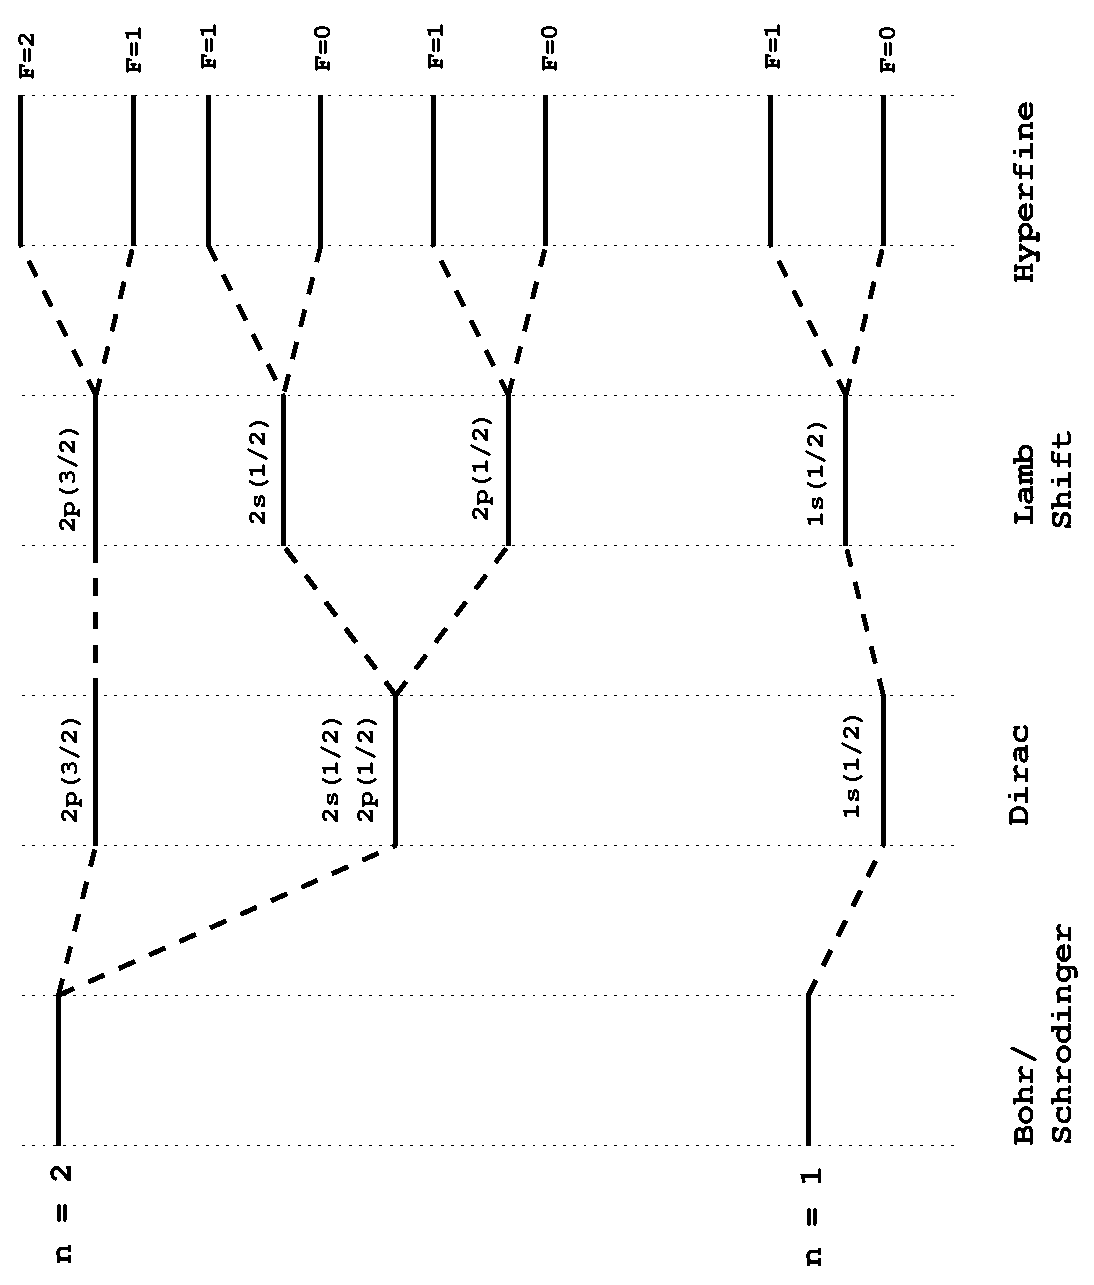
\includegraphics[angle=-90,width=0.6\textwidth]{all.eps}
    \end{frame} 

    %Figure~\ref{fig:split} shows the splittings of the different energy
    %in a Hydrogen atom for n = 1 and n = 2. The diagram is not to scale and
    %are magnified form the left to the right. The diagram qualitatively shows
    %the effect on the Bohr/Schr\"odinger energy from the various corrections
    %such as the Dirac fine structure, the Lamb Shift (described in the 
    %next section) and the hyperfine structure.

    \subsection{21 cm Line of Atomic Hydrogen}
    \begin{frame}{21cm Line of Atomic Hydrogen} 
        \begin{itemize} 
            \item The energy level splitting diagram in the previous figure shows that the ground state of
    the hydrogen atom splits into two hyperfine levels with the total angular
    momentum of the atom being $F=0$ and $F=1$.
\item The difference in energy between these two levels is 1420 MHz which corresponds
    to a wavelength of $\lambda \approx $ 21 cm. 
\item The probability of a transition occurring between these two levels is very low and occurs on average only 
    once every few million years. 
\item However, there is a large amount of hydrogen gas
    in the galaxy allowing radio telescopes easily detect this 21 cm transition and
    therefore allow the mapping of hydrogen in the galaxy.
        \end{itemize} 
    \end{frame} 

\section{Lamb Shift}
\begin{frame}{Lamb Shift} 
\begin{itemize} 
    \item    Investigation of the fine structure of hydrogenic atoms using spectroscopic techniques
    in the 1930's showed that there were small differences between the observed spectra
    and the theoretical predictions made by the Dirac equation.
    \item For example, according to the Dirac equation the $2s_{1/2}$ and the $2p_{1/2}$ states
    coincide at the same energy level. Observations showed that the $2s_{1/2}$ was shifted 
    slightly upwards by about 0.03 cm$^{-1}$.
    \item A very accurate measurement of the shift was made in 1947 by Lamb and Retherford using
    microwave techniques to stimulate a direct radio-frequency transition between the 
    $2s_{1/2}$ and the $2p_{1/2}$ levels. 
    \item This small shift of energy levels became known as the Lamb shift.
\end{itemize}
\end{frame} 

    \begin{frame}{Visualising the Lamb Shift} 
        \centering
        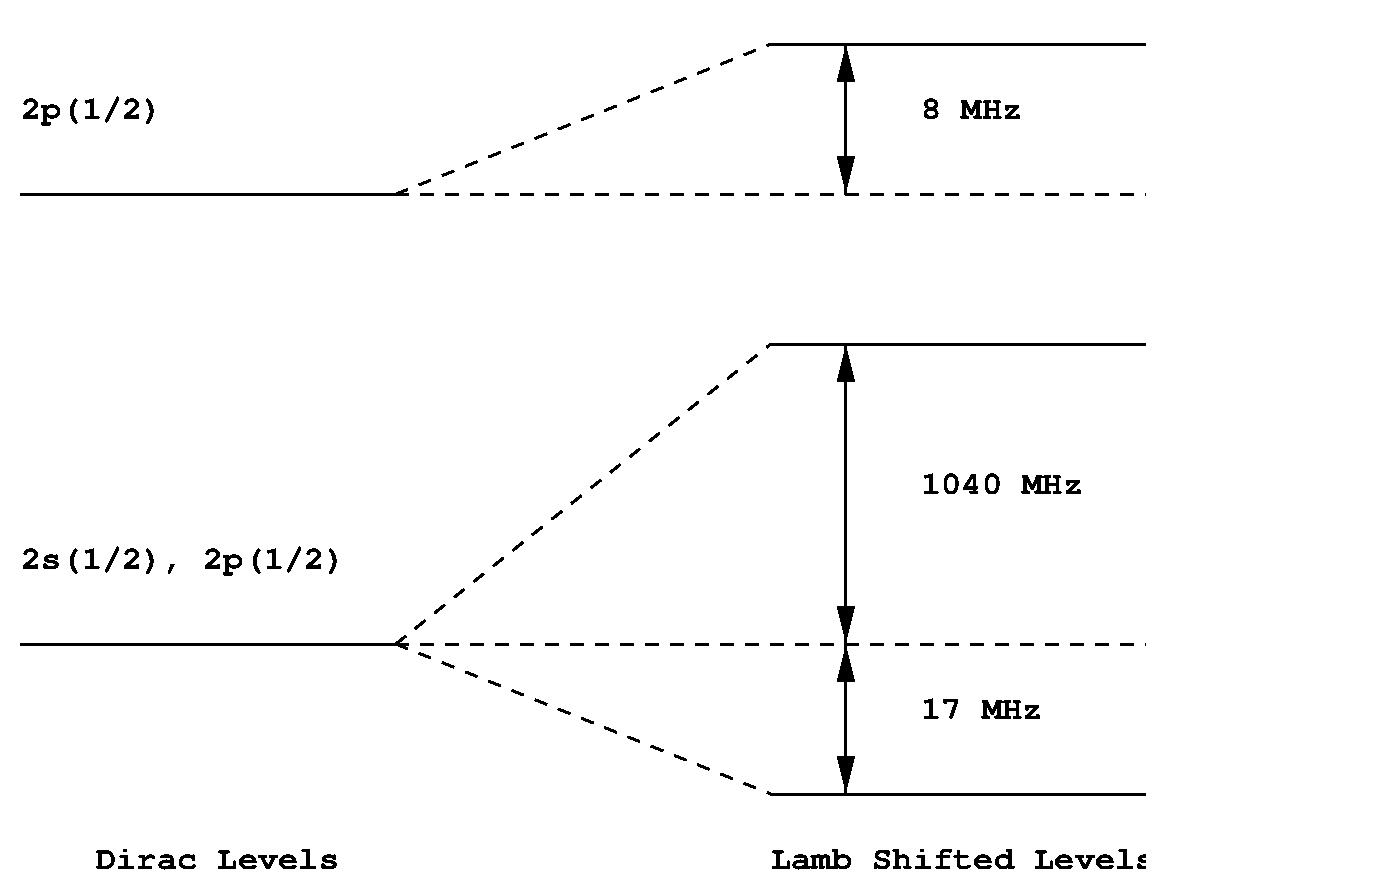
\includegraphics[width=0.8\columnwidth]{lamb.eps}
    \end{frame} 


    \begin{frame}{Quantum Electrodynamics}
        \begin{itemize} 
        \item The physics of the Lamb shift are described in the theory of quantum electrodynamics,
    in which radiative corrections to the Dirac equation are obtained by taking into
    account the interaction of a quantised electromagnetic field with an electron.

    \item The Lamb shift arises because of the zero point energy of a quantised electromagnetic
    field is non zero, similar to the zero point energy of a quantum harmonic oscillator.
    In a vacuum, fluctuations of the zero point energy of the quantised radiation field
    act on the electron. 
    \end{itemize} 
\end{frame} 

    \begin{frame}{Quantum Electrodynamics (2)} 
    \begin{itemize}     
    \item The effect of the electron is to cause it to oscillate rapidly
    about some equilibrium position. As a result of this oscillatory motion, the electron
    does not appear to be point charge -- instead the electron charge is slightly smeared
    at in a sphere of some small radius. 
    
    \item When the electron is bound by an electric field
    as it is in an atom, the potential it experiences is slightly different to that 
    experienced by the electron in it's mean position. 
    
    \item Therefore electrons which are
    most sensitive to short distance modifications such as those in the ground state
    are raised in energy with respect to other states to which the shift is much smaller.
        \end{itemize} 
    \end{frame} 

    \begin{frame}{References} 
    \begin{enumerate}
        \item \emph{Physics of Atoms and Molecules}, Bransden and Joachain
        \item \emph{Quantum Mechanics of One- and Two-Electron Atoms},
                    Bethe and Salpeter
        \item \emph{Intermediate Quantum Mechanics}, Bethe
        \item \emph{Advanced Quantum Mechanics}, Sakurai
        \item \emph{The Spectrum of Atomic Hydrogen - Advances}, Series
        \item \emph{Quantum Mechanics}, Merzbacher
        \item \emph{Modern Physics}, Serway, Moses and Moyer
        \item \emph{WikiMedia Commons} Hydrogen Spectrum \\
            \url{http://commons.wikimedia.org/wiki/File:Hydrogen_spectrum.svg} 
    \end{enumerate}
    \end{frame} 

\end{document}
